\chapter{Theory}\label{theory_part}
This chapter goes through the various techniques used in image processing. Here they are describe in general, while chapter \ref{implementation} will show how they were used for this specific project.

\section{A general framework for image processing}
Image processing can be described as an umbrella term. \citep{ip_book} writes that Image processing comes from the general field of signal processing, and that it covers ways to segment objects of interest on a digital image. This is achieved using multiple steps. It should be noted, however, that the order of the steps sometimes change, and there might be more focus on some than others. That being said, this is a general framework that can be used as a good starting point (based on \citep{ip_book}):

\textbf{Image Acquisition}
Before anything can be processed, data needs to be captured, typically using a camera. This step is all about the setup, as well as the environment, setting, light, etc.

\textbf{Pre-processing}
Here the initial setup is completed, e.g. converting the image from color to grayscale.

\textbf{Segmentation}
To be able to work with a specific object, for instance a hand, it needs to be separated from the rest of the picture. This is done using segmentation where noise and background elements are removed, so only the object of interest is seen. Thresholding is often applied to make the object stand out, e.g. make the object appear white and the background black.

\textbf{Representation}
The object needs to be representative in an intuitive manner.

\textbf{Classification}
For the system to actually know that an object is a hand or not, it has to do some classification and compare the data to some knowledge or database. This can be done with template matching and BLOB classification.

Figure \ref{fig:ip_framework} illustrates the framework used typically when working with image processing.

\begin{figure}[htbp]
\centering
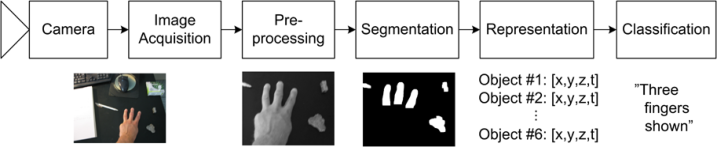
\includegraphics[width=1.00\textwidth]{Pictures/Theory/imageProcessing_steps.png}
\caption{Image Processing framework. - WE SHOULD MAKE OUR OWN PICTURE LATER ON!!!!!!!! - Gustav}
\label{fig:ip_framework}
\end{figure}

%% Maybe a little to blabla and too long sentences - Gustav %%
During this project image processing has been used achieve an the output needed. Some techniques is being used to remove noise from the picture, so the important parts get all the focus, while others are used for making the important parts more clear or making it possible to track specific objects.

It is all these different techniques combined that makes it possible to get a functional program, but before you can use them, you will have to know how they work and how they can be included to your project. This section is going to explain the different techniques that are being used and also why and how they are being implemented in this project.

\section{The digital Image}
Working around digital images on computers is something that most can relate to, but there is a lot more to it than one realizes. Figure \ref{fig:ip_ColoredToGrayscaleToBinary} shows what this chapter is all about; working with color, grayscale or binary images, and the different attributes of each type.

\begin{figure}[htbp]
\centering
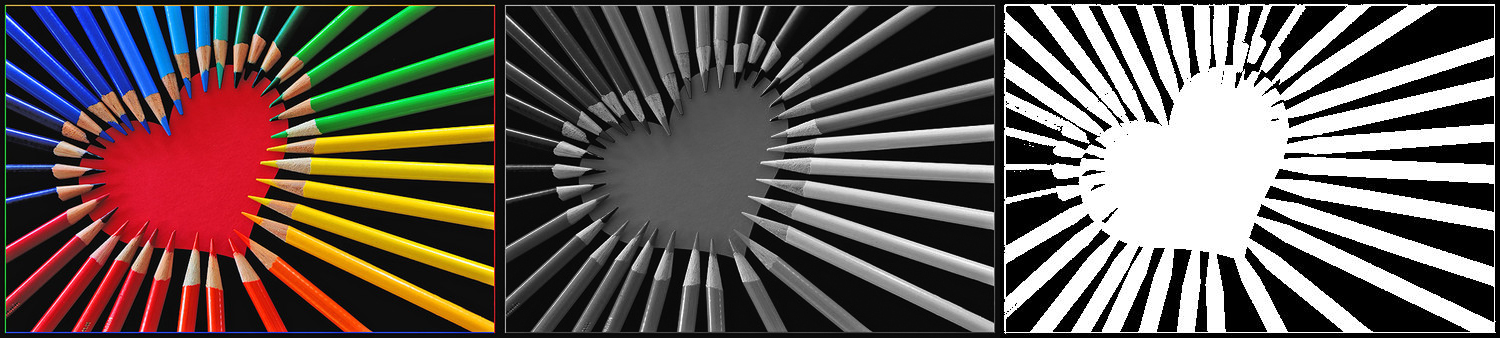
\includegraphics[width=1.00\textwidth]{Pictures/Theory/ColoredToGrayscaleToBinary.jpg}
\caption{Image illustrating a conversion from a colored image to grayscale and finally to binary}
\label{fig:ip_ColoredToGrayscaleToBinary}
\end{figure}

\subsection{Pixels}
[Need to write what a pixel is. Use IP book.]

\subsection{8-bit image and grayscale images}
In an 8-bit image, the 8-bit prefix describes the \textit{bit depth} of the image. The bit depth tells us about the amount of information there can be stored in a single pixel.

An image with a single channel of information for each pixel in the X and Y axis is typically a grayscale image, since each pixel is limited to information about a single hue \fixme{define hue - use IP book}. The information stored in each pixel is the intensity \fixme{define intensity - IP book} of the particular pixel. 8 bit evaluates to $2^8$ different states, meaning that a single 8-bit pixel can display 256 different levels of intensity, or in the case of a zero-based computer system, 0-255 (see figure \ref{fig:ip_grayscale}). An 8-bit image is a widely-used format for images, but it is also possible to create images with more depth and with more information for each individual pixel. Examples of that are images in 16 and 32 bits. A 16-bit depth is equal to $2^{16}$ different states, which means that each pixel can hold any one of 65,536 different shades of gray. Simultaneously, a 32-bit depth is equal to $2^{32}$, which gives 4,294,967,296 different shades of gray.

\begin{figure}[htbp]
\centering
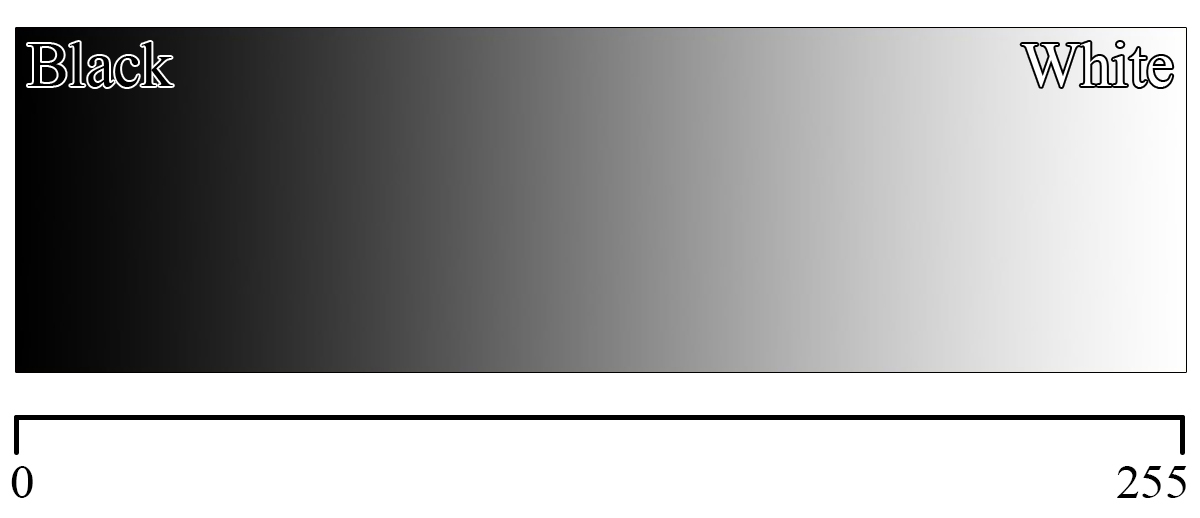
\includegraphics[width=0.7\textwidth]{Pictures/Theory/Grayscale.jpg}
\caption{Image illustrating the 256 different gradients of an 8 bit picture.}
\label{fig:ip_grayscale}
\end{figure}
 
\subsection{Indexing an image}
When working with images on a computer and performing image processing, one often has to look at the individual pixels within an image.

Working with pixels in a image is like working with a coordinate system. Starting in the top-left corner is (0,0). Going to the right, the X value increases; going down, the Y value increases. A single pixel can be described as a coordinate, e.g. (255,255) is the bottom-most corner to the right. Figure \ref{fig:ip_IndexingAPicture} illustrates this.

\begin{figure}[htbp]
\centering
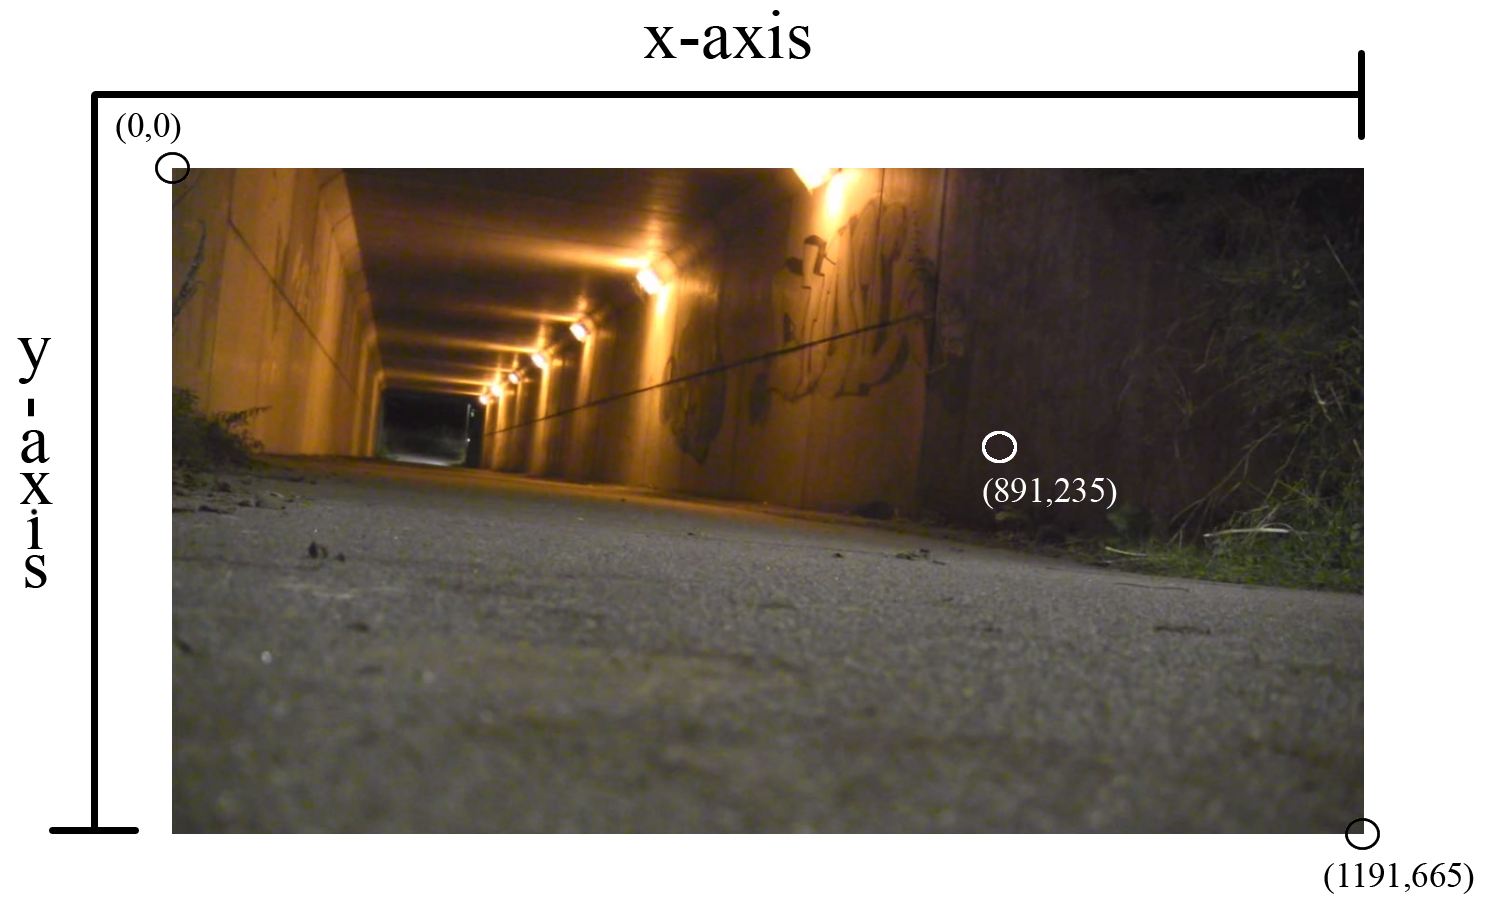
\includegraphics[width=1.00\textwidth]{Pictures/Theory/IndexingAPicture}
\caption{The pixel values are stored in a coordinate system. Note that Y goes down and not up.}
\label{fig:ip_IndexingAPicture}
\end{figure} 

In OpenCV, images are stored in a matrix (see figure \ref{fig:opencv_matrix}) . The size of the matrix holding the pixel values of the X and Y axis is as wide as the proportions of the image, therefore, when an image with a resolution of \textit{1024*1024} pixels is loaded, the highest coordinate assigned to pixels in the the matrix is (1023,1023).

\textbf{[WE NEED TO DESCRIBE OPENCV MATRICES BETTER!!!]}

\begin{figure}[htbp]
\centering
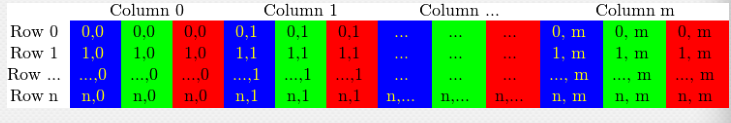
\includegraphics[width=1.00\textwidth]{Pictures/Theory/opencv_matrix}
\caption{OpenCV stores the pixel values in a matrix system. - [NEEDS SOURCE / THEODORE!!!]}
\label{fig:opencv_matrix}
\end{figure} 

%%% GUSTAV NÅEDE HERTIL TIRSDAG 4. DECEMBER 2012, 17:36 %%%
%%% GUSTAV NÅEDE HERTIL TIRSDAG 4. DECEMBER 2012, 17:36 %%%
%%% GUSTAV NÅEDE HERTIL TIRSDAG 4. DECEMBER 2012, 17:36 %%%
%%% GUSTAV NÅEDE HERTIL TIRSDAG 4. DECEMBER 2012, 17:36 %%%
%%% GUSTAV NÅEDE HERTIL TIRSDAG 4. DECEMBER 2012, 17:36 %%%
%%% GUSTAV NÅEDE HERTIL TIRSDAG 4. DECEMBER 2012, 17:36 %%%
%%% GUSTAV NÅEDE HERTIL TIRSDAG 4. DECEMBER 2012, 17:36 %%%
%%% VVVVVVVVVVVVVVVVVVVVVVVVVVVVVVVVVVVVVVVVVVVVVVVVVVV %%%
\subsection{Working with coloured images}
Now that a basic knowledge regarding images has been established, the next step into using images in calculations is to understand the basics of a coloured image.\\
There are several formats for handling color images. In this report we will only decribe RGB, since this is the only format we will encounter. Compared to a grayscale image, a coloured image differs because it consists of 3 channels, opposed to just one channel in grayscale images. Each of the three channels describe the value of the color in the specific pixel in relation to red, blue or green, which are the primary colors our eyes are sensitive to. The most significant difference between grayscale images and coloured images, is that one would not describe the intensity of one specific color, but a mix of the red, green and blue color. In addition equal amounts of red, green and blue  will produce a gradient of grey, where a pixel value of 255 will produce white, and a pixel value of 0 would produce black, similar to grayscale images.\\
Knowing the specific values of the red, green and blue channels within an image gives the user a great advantage, especially when performing image manipulations in programming. If one wants to exclude a specific color in a mathematical operation, such as red, one would simply have to create a threshold\fixme{Insert footnote telling: "Threshold will be described later in the theory chapter, but means to segment a specific colour only and create a binary picture"} value to segment the pixels depending on values of the red channel. The outcome should be a picture with a limited/controlled amount of red. 

Figure \ref{fig:ip_ColorWheel} Illustrates the making of colors in relation to the RGB system.

\begin{figure}[htbp]
\centering
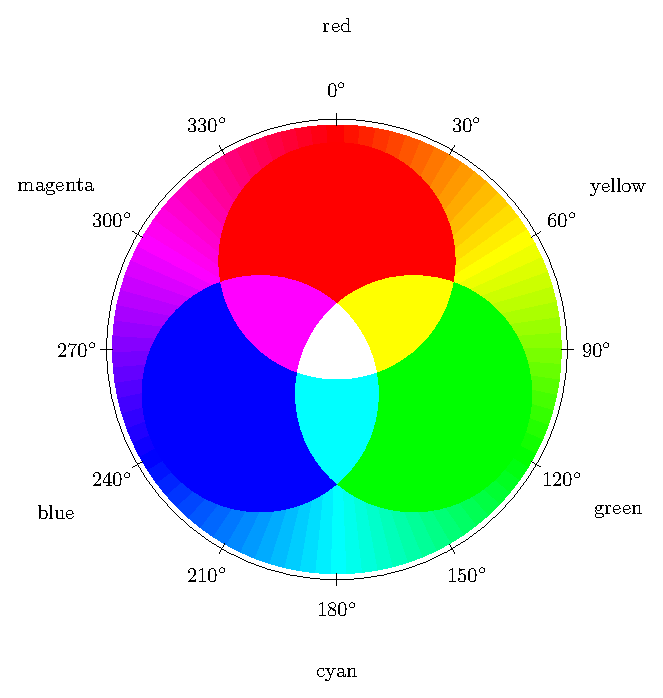
\includegraphics[width=0.50\textwidth]{Pictures/Theory/RGBColor.pdf}
\caption{Image illustrating the making of colors - \citep{colorMixing}}
\label{fig:ip_ColorWheel}
\end{figure} 

\subsection{Binary Images}
In comparison to the above-mentioned, where images are defined by bit depth and pixel information, binary pictures is represented by two colors only in form of black and white. Using this often correlates to use of a threshold, described in section \ref{sec:Thresholding}. Binary pictures are less resource demanding when performing mathematical operations as each pixel only can take one of two values.\\
Using the tool correctly, one will be able to adjust the input so that only usable pixel information remains in the picture. However one should be careful when using thresholding, as it's easy to over- and undersegmentate an input. More about this in the next section.


%%% I SKIPPED THIS BECAUSEI WROTE IT MYSELF - JOE 5/12 - 2012 %%%
%%% I SKIPPED THIS BECAUSEI WROTE IT MYSELF - JOE 5/12 - 2012 %%%
%%% I SKIPPED THIS BECAUSEI WROTE IT MYSELF - JOE 5/12 - 2012 %%%
%%% I SKIPPED THIS BECAUSEI WROTE IT MYSELF - JOE 5/12 - 2012 %%%
\section{Thresholding}
\label{sec:Thresholding}
Thresholding is one of the most fundamental operations in point processing \fixme{WHAT is point processing? - Gustav} and it is performed to make an input picture binary, i.e. either black, which relates to the pixel value of 0 or white, which relates to the pixel value of 255. Making an image binary means to show the image in only completely black and completely white pixel values. \\
This is useful in programs where you need to find silhouettes, such as tracking a person, where smaller details are not of importance.\\
To determine which pixels that should be completely black and which that should be completely white a fixed thresholding value is required. Using a metaphor, the threshold value can be compared to a gatekeeper that lets everyone who is 18 years old or older inside the club, but denies access to people who are 17 or younger. Using this analogy; pixels that are "old" (bright) enough are let in, while "younger" pixels (dark) are denied.

Using the same analogy that somebody decided that the border between being too young and just old enough, should be 18 years. This age could easily be something different, such as 17 or 24. The same is relevant with thresholding. You have to decide when pixels are "old" enough (bright). If they are too young (dark), they cannot get access.

In practice this means that pixels with values greater than a threshold is set to TRUE (or white), which typically is 255 when talking in bytes. On the other hand, if a pixel is less than the threshold value, it is set to FALSE (black) or 0. To sum this up the formula for making a threshold is shown in equation \ref{threshold}.
\begin{equation}
  \begin{aligned}
  	\text{if } f(x,y)\leq T \quad \text{then } g(x,y)&= 0 \\
  	\text{if } f(x,y)>T \quad \text{then } g(x,y)&= 255
	\label{threshold}  
  \end{aligned} 
\end{equation}
Where $T$ is the threshold value, $f(x,y)$ is the input pixel and $g(x,y)$ is the output pixel. 

When setting the thresholding value it is important to think about what is wanted regarding the output. It differs  from image to image how effective thresholding is, based on the contrast difference between the object and the background. If the background, and the object you want to find are very different in color and/or contract, then it is easy to distinguish between them and choose an effective threshold value. However; if the object and background are very similar, it becomes harder to do choose a thresholding value. As you will have to chose between losing information associated to the object of interest or to gather some background noise, but then keeping the object of interest.\\
To get a better understanding of this, look at the histograms shown in \eqref{fig:SimpleThreshold} and \eqref{fig:ComplicatedThreshold} that shows to grayscale pictures.

It is easy to tell that the leftmost histogram is more ideal to threshold because the object and background are very different, while the rightmost histogram has very similar object and backgrounds.

\begin{figure}[htbp] \centering
\begin{minipage}[b]{0.45\textwidth} \centering
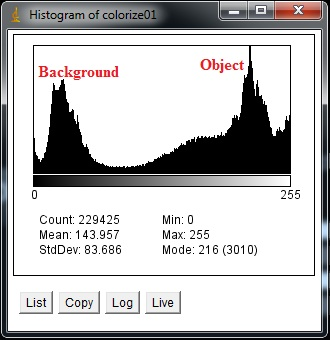
\includegraphics[width=1.00\textwidth]{Pictures/Theory/SimpleThresholdPicture} % Venstre billede
\end{minipage} \hfill
\begin{minipage}[b]{0.45\textwidth} \centering
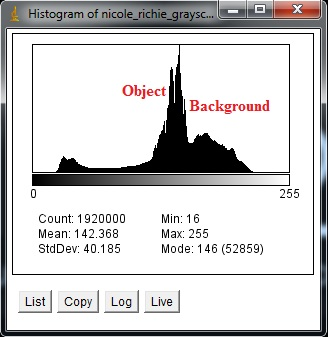
\includegraphics[width=1.00\textwidth]{Pictures/Theory/ComplicatedThresholdPicture} % Højre billede
\end{minipage} \\ % Captions og labels
\begin{minipage}[t]{0.45\textwidth}
\caption{Simple threshold value} % Venstre caption og label
\label{fig:SimpleThreshold}
\end{minipage} \hfill
\begin{minipage}[t]{0.45\textwidth}
\caption{Complicated threshold value} % Højre caption og label
\label{fig:ComplicatedThreshold}
\end{minipage}
\end{figure}

Looking at picture \eqref{fig:SimpleThresholdAfter} will show that the picture with the leftmost histogram, figure \eqref{fig:SimpleThreshold}, gives a clear outline of the silhouette of a woman after the thresholding value is applied. However, looking at figure \eqref{fig:ComplicatedThresholdAfter} shows that the picture with the rightmost histogram, figure \eqref{fig:ComplicatedThreshold}, produces a poor silhouette of a woman, due to the fact that the background and the object has very similar colors. 

\begin{figure}[htbp] \centering
\begin{minipage}[b]{0.45\textwidth} \centering
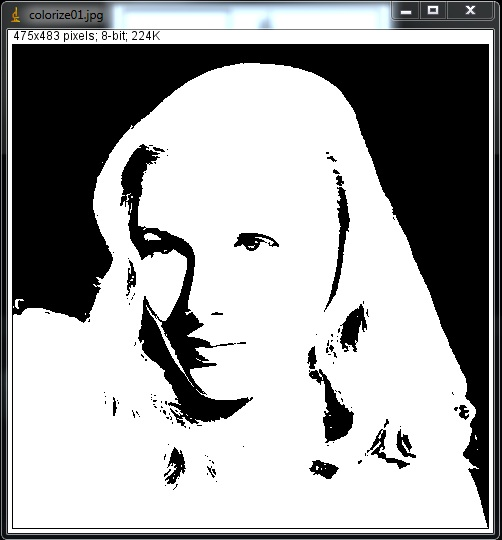
\includegraphics[width=1.00\textwidth]{Pictures/Theory/SimpleThresholdAfter} % Venstre billede
\end{minipage} \hfill
\begin{minipage}[b]{0.45\textwidth} \centering
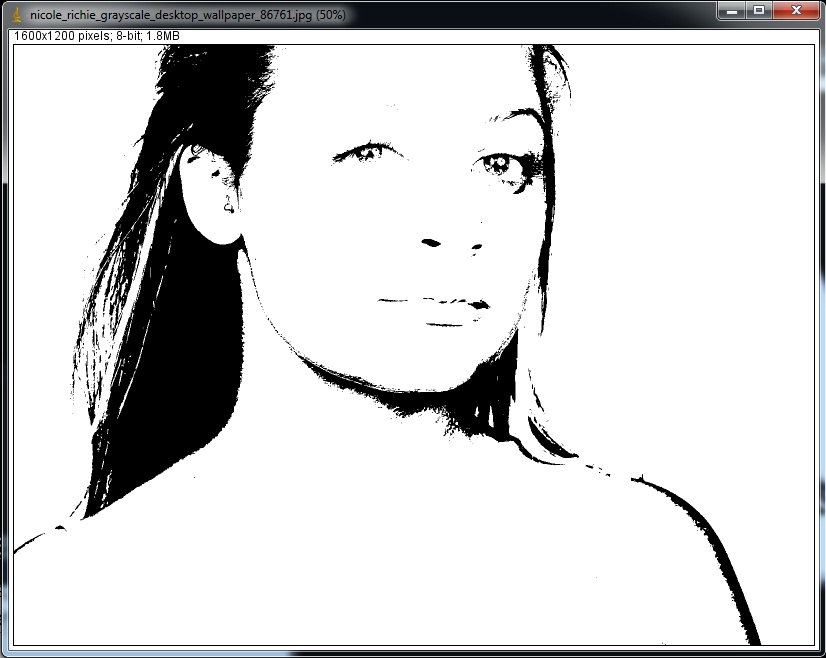
\includegraphics[width=1.00\textwidth]{Pictures/Theory/ComplicatedThresholdAfter} % Højre billede
\end{minipage} \\ % Captions og labels
\begin{minipage}[t]{0.45\textwidth}
\caption{Great silhouette after threshold} % Venstre caption og label
\label{fig:SimpleThresholdAfter}
\end{minipage} \hfill
\begin{minipage}[t]{0.45\textwidth}
\caption{Bad silhouette after threshold} % Højre caption og label
\label{fig:ComplicatedThresholdAfter}
\end{minipage}
\end{figure}
 
This proves the point that finding a functional thresholding value is not always straightforward. As for finding a silhouette it is of great help to make a clear transition from the object and the background.

\section{Morphology}
Morphology is a collection of operations used to analyse and process structures. Although these techniques is commonly used on binary images, it is possible to apply them to grayscale images as well.
The processes related to morphology on binary images are oriented to remove noise produced by threshold of an image as well as defining the contours of the objects in order to achieve a proper BLOB analysis.

Mathematical morphology is a neighborhood processing method\fixme{Is this the right way to describe it, or "home made"?} that applies a \textit{structuring element} (or kernel) to the pixels on the image. The ways that kernel will be structured, how big it will be or the shape that will be used, depends on the designer\fixme{There must be some boundaries or some predefined kernels? These should be described so the reader doesn't think that the designer can make whatever kernel he wants.} and the shape and size of the objects to be analysed. The reason for this is that the structured elements are used to apply by \textit{hitting} or \textit{fitting} operations that will affect the results in different ways. Hit and fit will be described in the next section.

\subsubsection{Hit and Fit}
Whenever you decide to apply a structured element and \textbf{hit} the pixels, what you are actually doing is to calculate the value of the output pixel by comparing the values of the pixels on the input image and the kernel. A kernel is a sort of grid that has some values within it. These values are either 1 or 0 if used on a binary pixel. Dependent on these values and the images pixel values different output occurs.

The kernel will be first placed on the corner of the image and it will operate on one pixel at a time. If one of the pixels inside the kernel are "1" where the kernel is "1" as well then it hits. This means that the pixel in the center of the kernel will become a "1" in the output. If none of the pixels inside the kernel "hits" then the pixel in the middle of the kernel becomes a "0" in the output.

\begin{figure}[htbp]
\centering
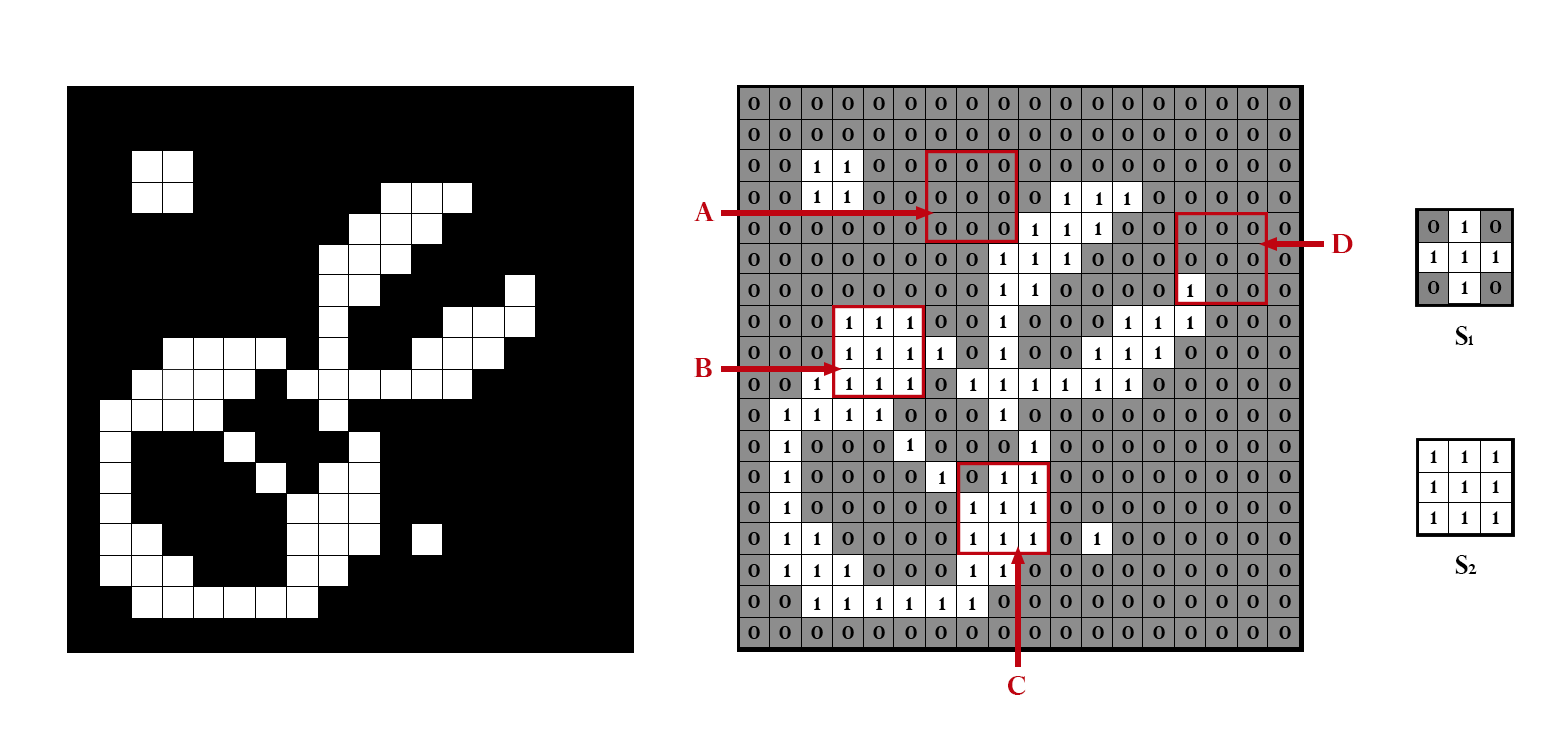
\includegraphics[width=1\textwidth]{Pictures/Theory/FitHitKernels.png}
\caption{Binary image and \textit{Structuring elements}}
\label{fig:FitHit}
\end{figure}

On the contrary, to be able to \textbf{fit} a pixel on the center of the structured element, every pixels' values have to be the same both on the kernel and the input image. If one of the pixels on the input image has a different value to the corresponding '1's of the kernel, the pixel in which the kernel is centred will be a '0' on the output image. On Table \ref{tab:HitFitResults} Figure \ref{fig:FitHit} has been represented with two different types of structuring elements.
\begin{table}[htbp]
\centering
\begin{tabular}{|c|c|c|c|}
\hline
 \:Position\: &SE &\:\:\:Hit\:\:\: &\:\:\:Fit\:\:\: \\\hline
 \hline
 A &$S_{1}$ &No &No\\\hline
 A &$S_{2}$ &No &No\\\hline
 B &$S_{1}$ &Yes &Yes\\\hline
 B &$S_{2}$ &Yes &Yes\\\hline
 C &$S_{1}$ &Yes &Yes\\\hline
 C &$S_{2}$ &Yes &No\\\hline
 D &$S_{1}$ &No &No\\\hline
 D &$S_{2}$ &No &No\\\hline
\end{tabular}
\caption{Results of Hitting and Fitting with two different structuring elements}
\label{tab:HitFitResults}
\end{table}

%%%%%%%%%%%%%%%%%%%%%% SHOULD I TALK A BIT MORE ABOUT THE TABLE? %%%%%%%%%%%%%%%%%%%%%%%%%%%%
%%%%%%%%%%%%%%%%%%%%% NO - from Joe %%%%%%%%%%%%%%%%%%%%%%%%%%%%%
\subsection{Dilation}
Dilation is the process of applying Hit to an entire image and refers to the expansion of an object on an image (see Eq.\ref{Dilation1} for a mathematical definition). The result of this method implies helps filling small holes and merging objects. As mentioned before, the final effect on these objects will depend on the structured element (how big it is and which shape it has), this can be seen on Figure \ref{fig:Dilation}. 
\begin{equation}
\begin{aligned}
{g(x, y)}={f(x,y)}\oplus{SE}
\label{Dilation1}
	\end{aligned}
\end{equation}
A small structured element applied several times will have the same effect as a big structured element passed once. This can be seen on Eq \ref{Dilation2}, where dilating twice with the element {$SE_{1}$} has the same consequences on the object as dilating one time with {$SE_{2}$}, even though the only difference between those two kernels is that {$SE_{2}$} has a radius twice times bigger than the radius of {$SE_{1}$}.
\begin{equation}
\begin{aligned}
{f(x,y)}\oplus{SE_{2}} \approx ({f(x,y)}\oplus{SE_{1}})\oplus{SE_{1}}
\label{Dilation2}
	\end{aligned}
\end{equation}
%%%%%%%%%%%%%%%%%%%%%%%%% IMAGES WITH DILATIONS %%%%%%%%%%%%%%%%%%%%%%%%%%%%%%%%%%%%
\begin{figure}[htbp]
\centering
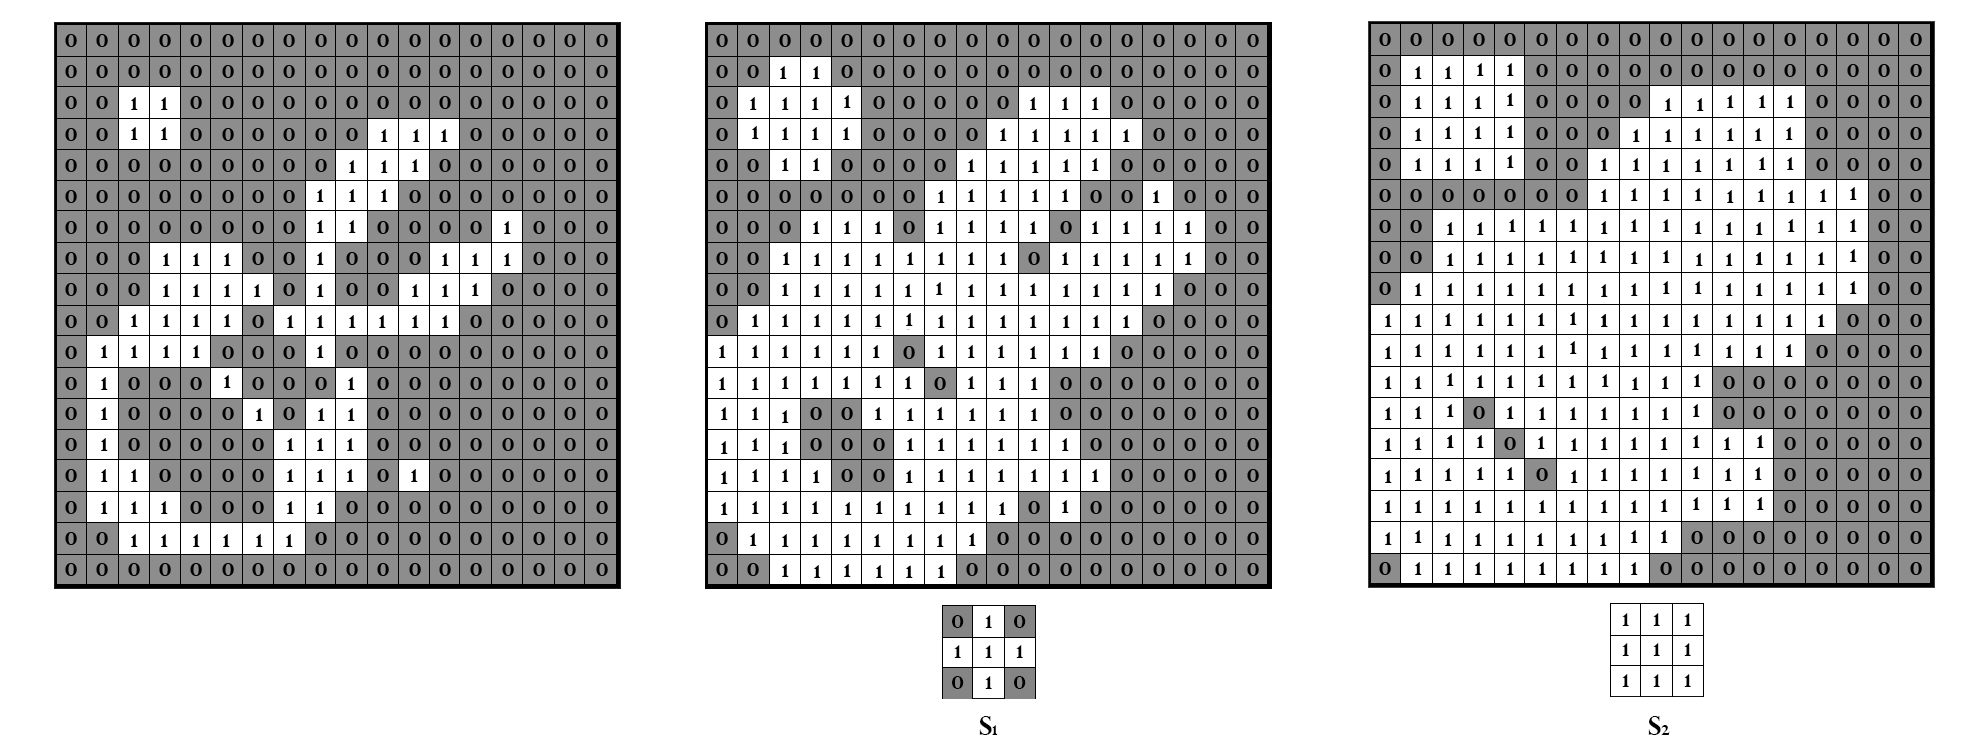
\includegraphics[width=1\textwidth]{Pictures/Theory/Dilation.png}
\caption{Dilation produced by two different structuring elements.}
\label{fig:Dilation}
\end{figure}

\subsection{Erosion}
The Erosion is the process of applying Fit to an entire figure and refers to the reduction of the size of an object in an image (the mathematical definition is provided on Eq. \ref{Erosion1}). As the Fit method is applied, small objects will also disappear and larger objects will be break down into smaller ones. As occurring with Dilation, the effects depend on the size, shape and values of the structured element. An example of \textbf{erosion}
\begin{equation}
\begin{aligned}
{g(x, y)}={f(x,y)}\ominus{SE}
\label{Erosion1}
	\end{aligned}
\end{equation}

%%%%%%%%%%%%%%%%%%%%%%%%% IMAGES WITH EROSIONS %%%%%%%%%%%%%%%%%%%%%%%%%%%%%%%%%%%%
\begin{figure}[htbp]
\centering
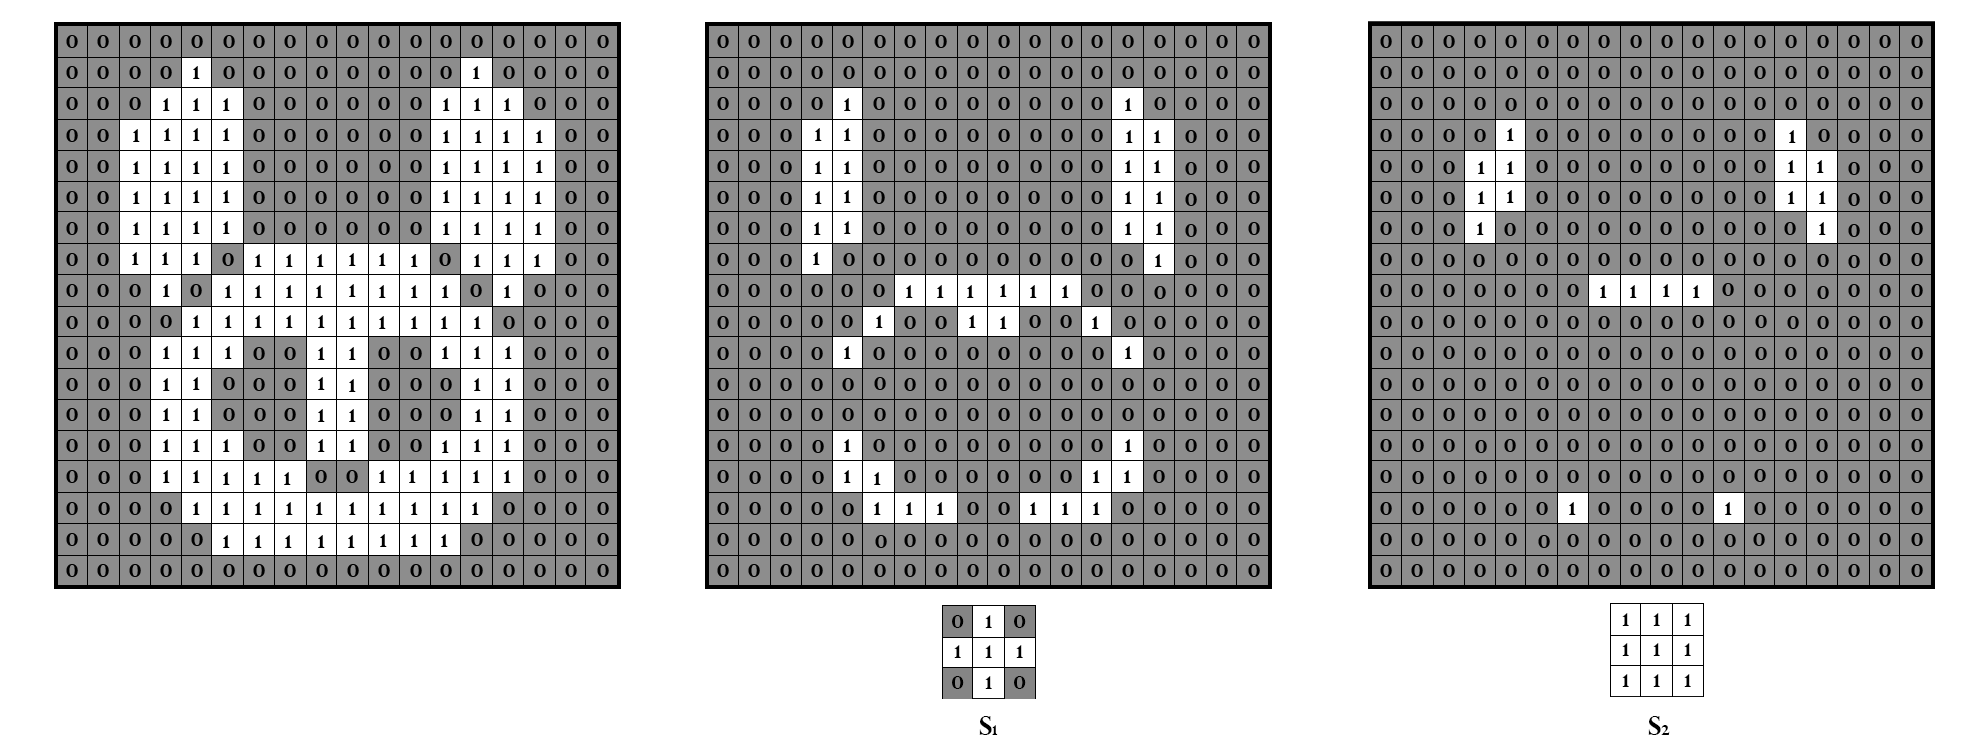
\includegraphics[width=1\textwidth]{Pictures/Theory/Erosion.png}
\caption{Erosion produced by two different structuring elements.}
\label{fig:Erosion}
\end{figure}

\subsection{Compound operations}
The term Compound Operations refers to the combination of dilating and eroding objects on an image and can therefore imply the \textit{Union} or \textit{Intersection} of the objects, but also other operations like \textit{Closing}, \textit{Opening} or doing edge detection, also know by \textit{Boundary detection}.
\subsubsection{Opening}
When \textit{eroding} images to erase small noise objects or split parts, it often occurs that the object of interest has decreased its size. The solution to this problem passes by dilating the eroded object. This operation is denoted \textit{Opening} and its mathematical definition is
\begin{equation}
\begin{aligned}
{g(x,y)}={f(x,y)}\circ{SE}=({f(x,y)}\ominus{SE})\oplus{SE}
\label{Opening}
	\end{aligned}
\end{equation}
The effect of Opening can be appreciated on Fig. \ref{fig:Opening}, where a circular kernel is applied to the image. Even though the object still conserves its original size, some information has been lost due to the effect of eroding and dilating the image, even if the same structured element is used along the process.

%%%%%%%%%%%%%%%%%%%%%%%%%%%%%%%%% INSERT OPENING IMAGES %%%%%%%%%%%%%%%%%%%%%%%%%%%%%%%%%%%%%
\begin{figure}[htbp]
\centering
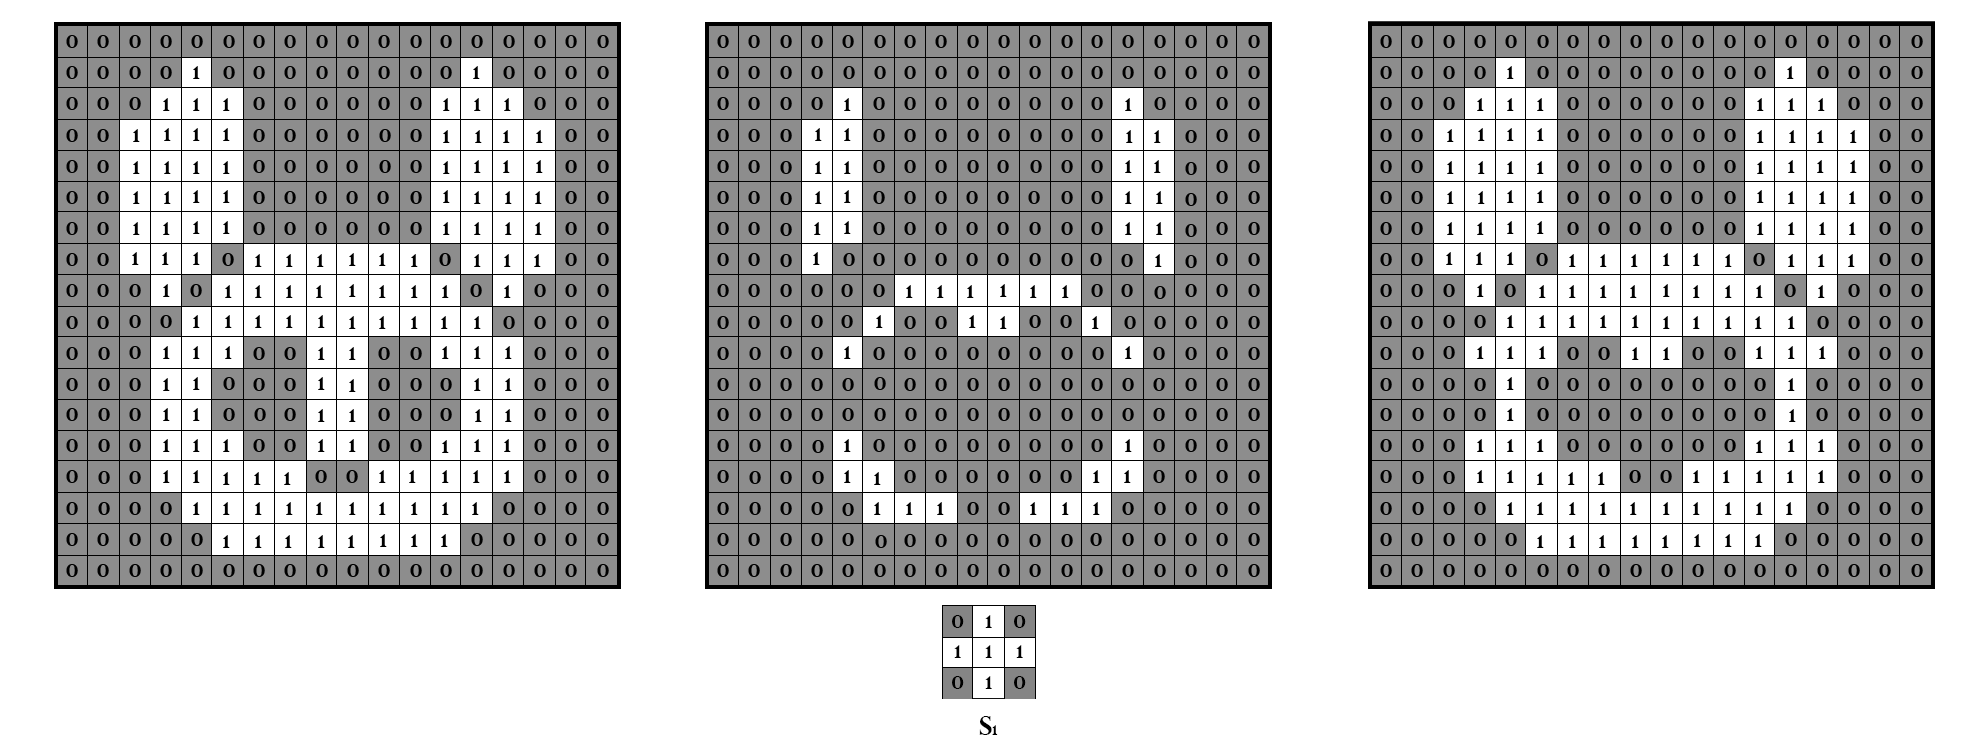
\includegraphics[width=1\textwidth]{Pictures/Theory/OpeningCirc.png}
\caption{Opening produced by a circular structured element.}
\label{fig:Opening}
\end{figure}

\subsubsection{Closing}
Another situation that often occurs when applying these methods comes from \textit{dilating} objects. When the size of the object is increased but it is still important to constrain the measure as well as filling the holes of the objects, a good solution will be to Erode after the Dilation. This is what Closing stands for and it is denoted by the formula \ref{Closing}. As with the Opening method, the size and shape of the kernel must be the same in order to obtain the desired result.
On Fig. \ref{fig:Closing} we can observe the effect of this operations: even though the holes are filled and the object maintains its original size, the noise of the background is still there. Therefore, it will be necessary to apply either Closing or a BLOB analysis method to delete those small objects.
\begin{equation}
\begin{aligned}
{g(x,y)}={f(x,y)}\bullet{SE}=({f(x,y)}\oplus{SE})\ominus{SE}
\label{Closing}
	\end{aligned}
\end{equation}
It is also important to remember that we can imply the Closing or Opening methods only one time. Most of the holes of the image will be filled but the size of the object will be the original one. If these operations are applied a second time, the size of the final image will be decreased or increased respectively.

%%%%%%%%%%%%%%%%%%%%%%%%%%%%%%%%%%% IMAGE CLOSING %%%%%%%%%%%%%%%%%%%%%%%%%%%%%%%%%%%%
\begin{figure}[htbp]
\centering
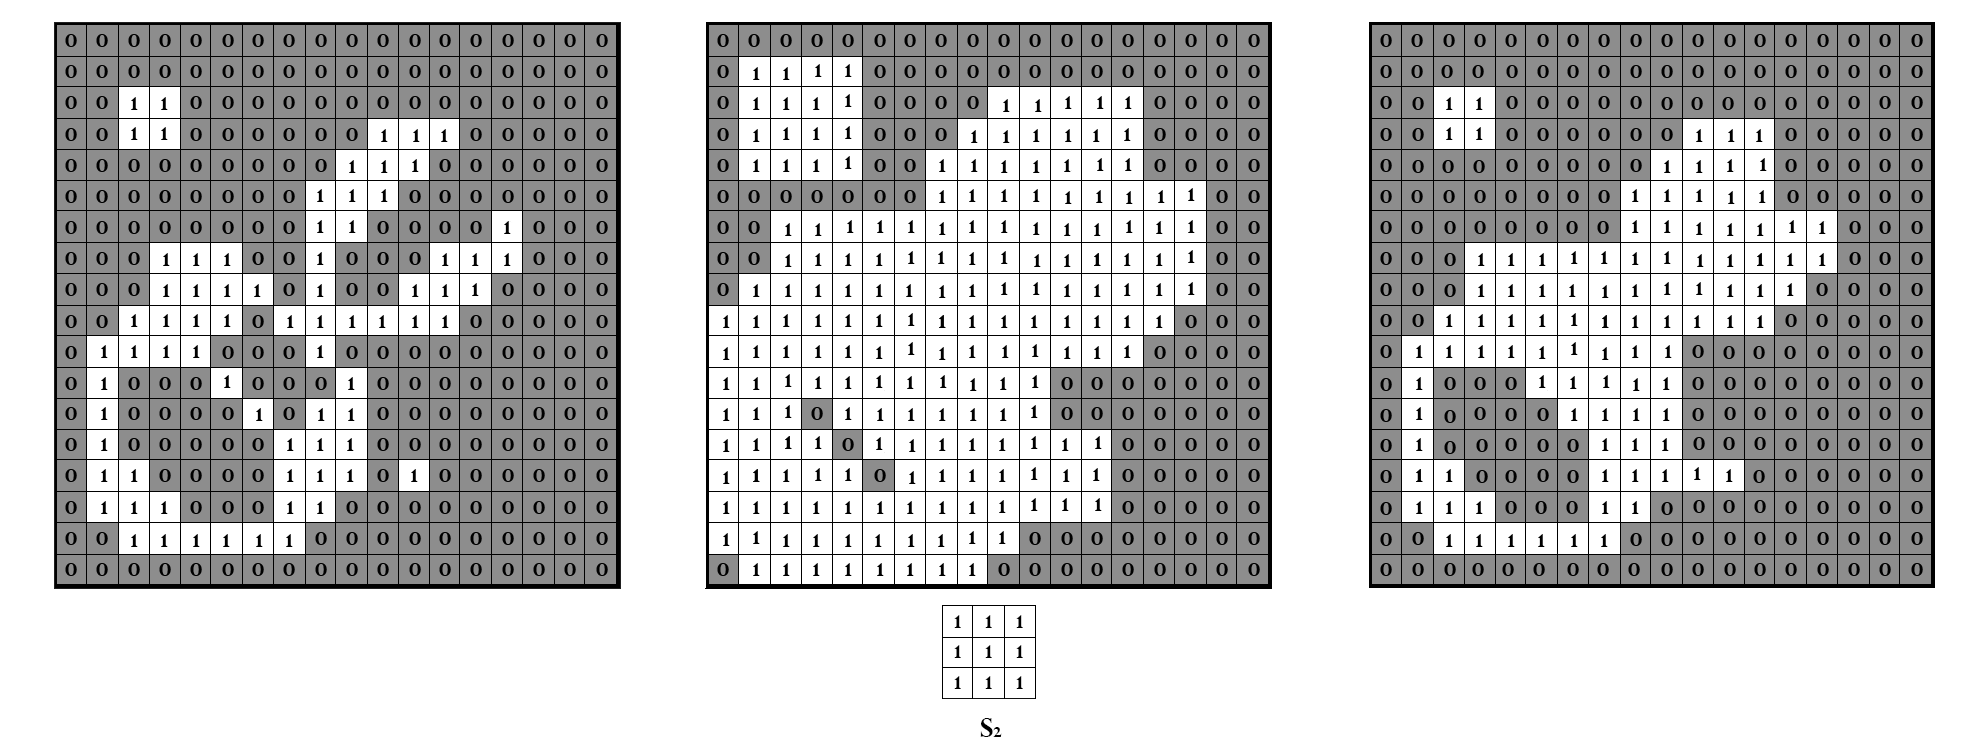
\includegraphics[width=1\textwidth]{Pictures/Theory/ClosingSq.png}
\caption{Closing produced by a squared structured element.}
\label{fig:Closing}
\end{figure}

\subsubsection{Boundary detection}
An alternative approach to the edge detection on binary images is the denoted \textit{Boundary Detection}. The performance of this operations is a compound of \textit{erosion} and \textit{subtraction}. Hence the first operation will be eroding the object to get a smaller version of it and then subtract it to the original input image so as to get a final output image with the border of the object. The mathematical definition of these operations is
\begin{equation}
\begin{aligned}
{g(x,y)}={f(x,y)}-({f(x,y)}\ominus{SE})
\label{BoundDetec}
	\end{aligned}
\end{equation}
When the purpose of implementing these operations is to find the edges, it is important to remember to apply dilation or erosion before, to remove the noise of the image. The results can be noted on Fig. \ref{fig:Boundary}, where the final result is a thin edge of the object.

%%%%%%%%%%%%%%%%%%%%%%%%%%%%%%%%%%% IMAGE SUBTRACTION %%%%%%%%%%%%%%%%%%%%%%%%%%%%%%%%%%%%
\begin{figure}[htbp]
\centering
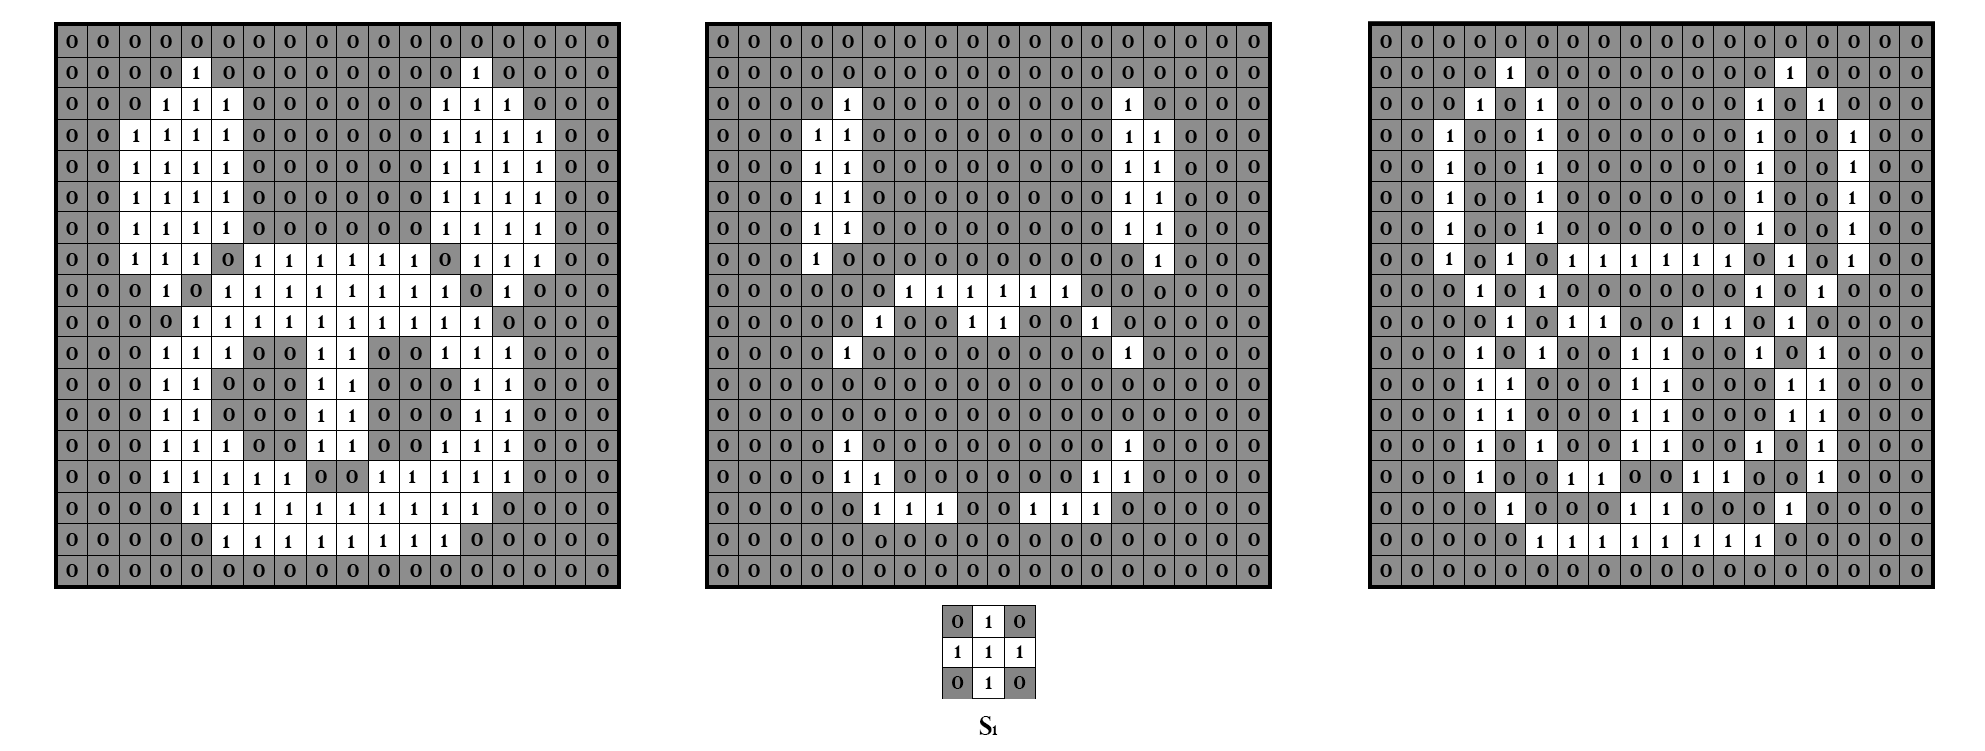
\includegraphics[width=1\textwidth]{Pictures/Theory/BoundaryEdges_circ.png}
\caption{Result of subtracting an eroded picture to the original one with a circular structured element.}
\label{fig:Boundary}
\end{figure}

%%% JOE GOT HERE 5/12 - 2013!!! %%%%%
%%% JOE GOT HERE 5/12 - 2013!!! %%%%%
%%% JOE GOT HERE 5/12 - 2013!!! %%%%%
%%% JOE GOT HERE 5/12 - 2013!!! %%%%%
%%% JOE GOT HERE 5/12 - 2013!!! %%%%%
\section{Region of interest (ROI)}
The Region of Interest or just ROI is a great image processing tool to optimize the frame rate of a camera. Cameras are getting improved all the time and the quality and amount of pixels information are enhanced simultaneously.\\
Generally one would think that the more pixels, the better quality, and the better output. This should however be reconsidered. Having the opportunity to access several pixels is a great opportunity to produce some magnificent pictures, but when a computer makes image manipulations changes to a picture it has to run through every single pixel one at a time. This means that in fact it would mean a lot to decrease the amount of pixels the computer has to process.\\
Therefore using a technique called Region of Interest or "ROI", is often used to reduce the amount of pixels being processed. ROI takes a region in the picture that is of interest. This region is usually enclosed in a rectangle and only the pixels inside this rectangle is being processed. That means that all the pixels outside of the ROI is ignored and unnecessary processing is prevented.
An example of how this could be used is taking a photo where only the head is of interest. The head then appears as the region of interest and only the pixels within the rectangle is processed. This is illustrated on figure \eqref{fig:Region of Interest}. This figure illustrates how many pixels that can be ignored.

\begin{figure}[htbp] 
\centering 
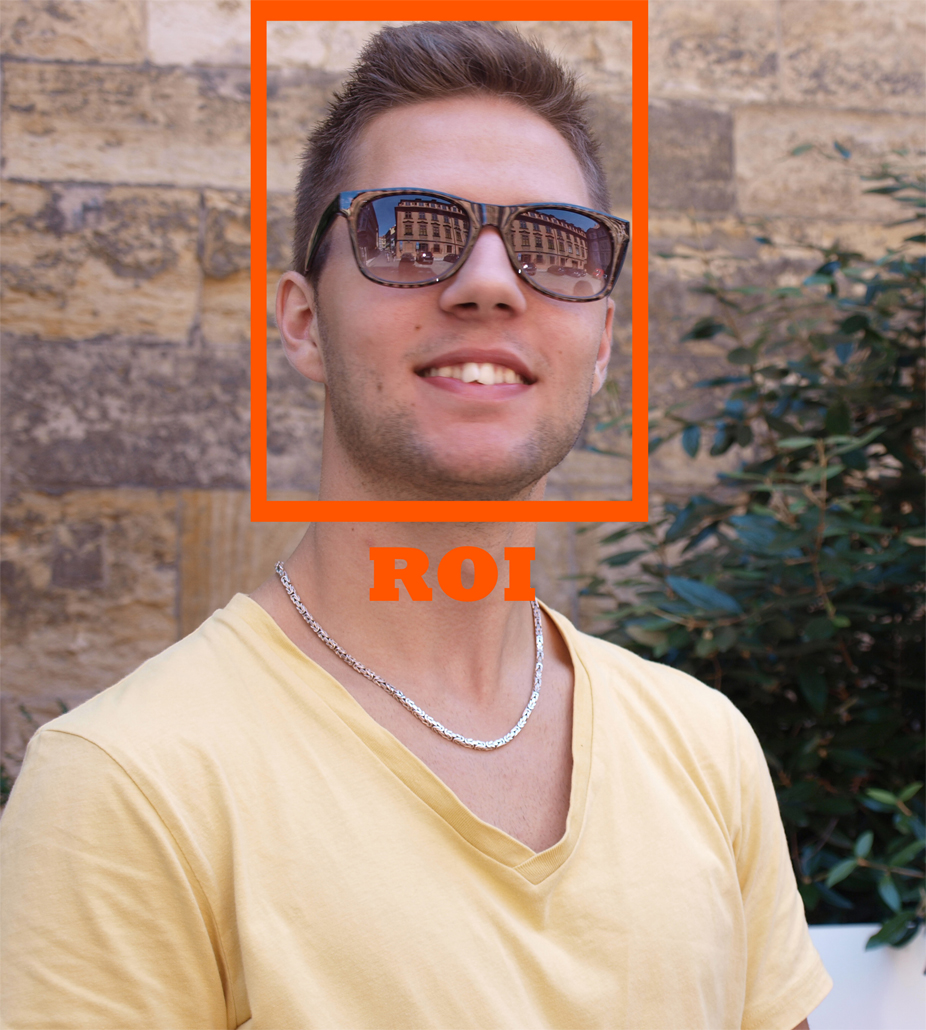
\includegraphics[width=0.5\textwidth]{Pictures/Theory/RegionOfInterest.jpg} 
\caption{Region of Interest} 
\label{fig:Region of Interest} 
\end{figure} 

\section{Background subtraction}
%% Working progress - Johannes %%
A way to detect changes in a scene and extracting an object is using background subtraction. As the name tells it is done by subtracting the background from the scene so only changes is being shown. Background subtraction is very efficient but unfortunately it is not always as simple as it sounds. \\
To be able to use background subtraction efficiently a controlled setup is required. The optimal setup is indoor with controllable light conditions. The setup is important because the background should not change. Imagine if sunshine is let inside a room. Then the light conditions will change together with the suns position, and changes will be seen everywhere spreading noise and giving an inaccurate result. \\
However, it is not realistic that each pixel in the background keeps the exact same pixel value all the time. Therefore a threshold value is required - for two reasons. First of all to make the changes in the scene more distinct from the background, but also to have a threshold value in which the background may vary. \\
Therefore the following two points has to be considered when doing background subtraction:
\begin{enumerate} 
	\item Is the background consistent? 
	\item Which threshold value would be optimal for making the picture binary, and distinct the changes from the background? 
\end{enumerate}

If the first point is false, and the background is not consistent then there is a way to automatically update the backgrounds pixel values. The formula is as following:

\begin{equation}
	\begin{aligned}
  		r_{new}(x,y)=\alpha*r_{old}(x,y)+(1-\alpha)*f(x,y)
		\label{AutomaticBackground}  
 	\end{aligned}
\end{equation}  

Where $r(x,y)$ is the reference image, $f(x,y)$ is the current image, and $\alpha$ is the weighting factor. The weighting factor $\alpha$ defines how fast the reference image updates. A typical weighting factor value is  $\alpha = 0.95$
\fixme{Insert reference - formula taken from page 70 in the Image Processing book}
Now that the background automatically updates, it is time to go to the next point.


If the background is consistent from the beginning then it also leads to the next point. 

The second point is about defining a threshold value. \\
To do this, it is necessary to check how much the backgrounds pixel values vary. This can be done by making a histogram for some random pixels in the background and check the values after recording some minutes. This should give an overview of how much the pixel values vary. Lets say that this procedure shows that an efficient threshold value is 20. This means that if a pixel in the background is of the intensity 80, then pixel values captured between the values $60-100$ will not make any changes, as it is thought as being the background. Pixels below 60 and above 100 will however be an object and be highlighted.
Another pixel in the background could have the intensity of 48 and the pixel values captured between $28-68$ would then be thought of as the background while values below 28 and above 68 would be seen as an object and be highlighted. \\
This type of threshold is a global threshold, which means that the threshold value is the same in every pixel in the scene. Imagine a scene where only part of the picture is being affected by lights. Then a unique threshold value for each pixel could be useful. This is possible using the following formula:

\begin{equation}
	\begin{aligned}
  		\ \text{Binary image} = \left\{ \begin{array}{ll}
         0, \quad &\text{if } Abs(g(x,y))<\beta * \sigma(x,y)\\
        255, \quad &\text{otherwise}.
        \end{array} \right . \ 
 	\end{aligned}
\end{equation} 

Where $\beta$ is the scaling factor, and $\sigma(x,y)$ is the standard deviation at the position $(x,y)$. Using this formula creates a local threshold.

When both points are considered, the background subtraction should be ready to use. In every frame in a scene each pixel will be checked for a possible change. If there is a change larger than what the threshold value allows then the pixel will be highlighted, revealing an object in the picture.

\section{BLOB analysis}
A common problem when dealing with images is to determine if the image data contains a particular object or shape. The term BLOB is an acronym for Binary Large Objects and refers to a region of connected pixels in a binary image. This technique is used to extract meaningful information from images. This is achieved by separating the pixels in points or regions that differ in properties like brightness or color changes (i.e., their value), and classifying them into one of two categories: the foreground (pixels with a non-zero value) and the background (pixels with a zero value).
Therefore, BLOB analysis will be split in three main steps: \textit{Extraction} of the BLOBs, \textit{representation} of the BLOBs and lastly, \textit{classification} of the BLOBs to know which ones belong to the expected type \citep{ip_book}.

\subsection{BLOB extraction}
To isolate BLOBs in a binary image, we need to define first if two pixels are connected or not. This is done by applying algorithms that will help to determine the connectivity of the pixels, but also the number of BLOBs contained in an image. The most commonly used kernels in BLOB extraction are the 8-connected and the 4-connected kernels. Where the 8-connected kernel is more accurate, but also requires more computations and consequently, needs more time to process the image and vice versa.

\subsubsection{Grass-Fire algorithm}
One of these connected component labelling algorithms is the \textit{Recursive Grass-Fire Algorithm}, used to erode images but also to track the pixels locations to create a region.
To explain this algorithm, we will use both 8-connectivity and 4-connectivity kernels to illustrate how these choices can affect to the final result.

\begin{figure}[htbp]
\centering
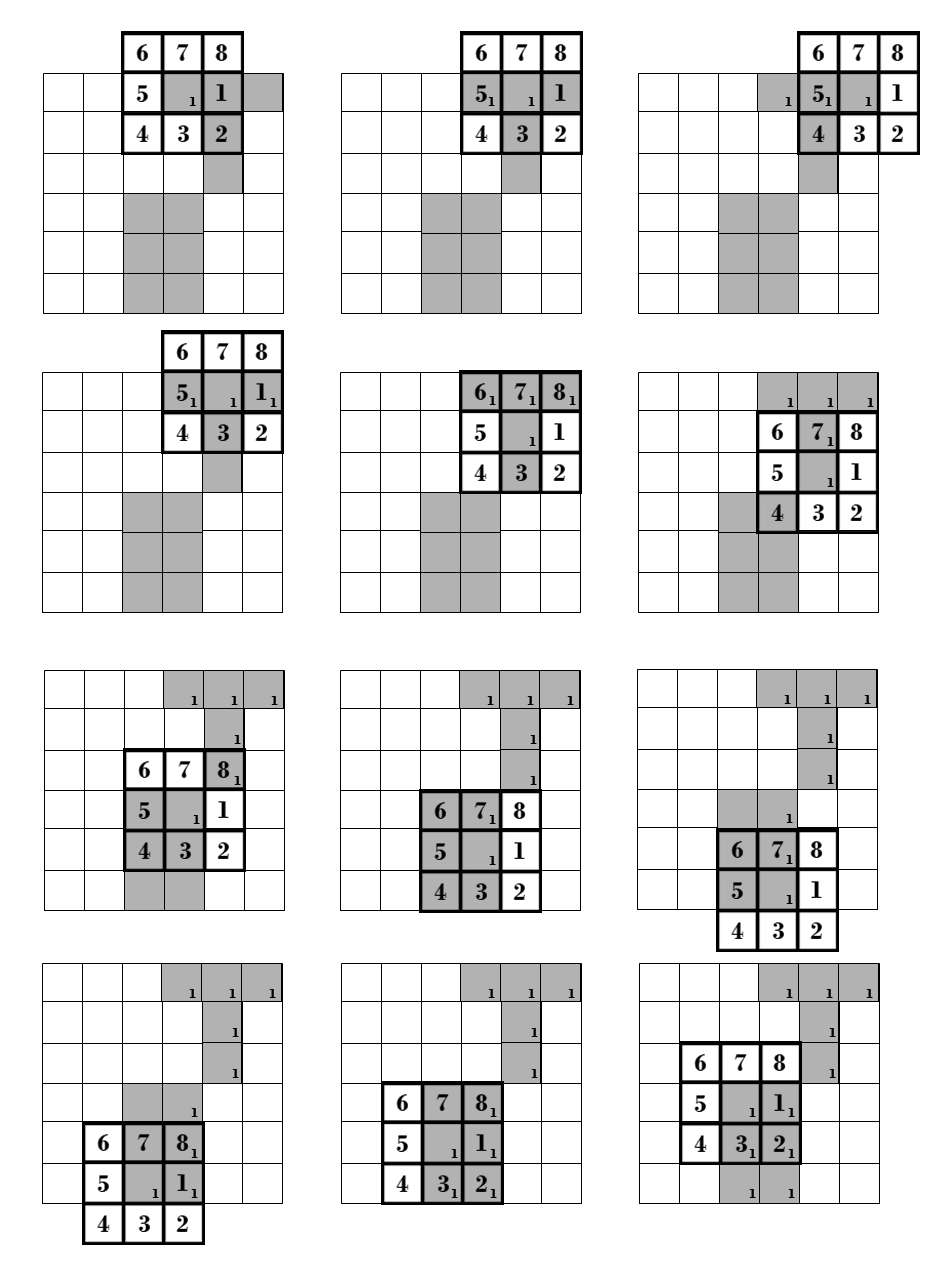
\includegraphics[width=0.8\textwidth]{Pictures/Theory/8connec_kernel.png}
\caption{8 connectivity labeling kernel detects 1 single object}
\label{fig:8connecK}
\end{figure}

As we can see on figure \eqref{fig:8connecK}, the Grass-Fire algorithm scans the entire image from the upper-left corner to the right bottom, row by row. When the kernel encounters a non-zero pixel value it centers on it and burns the center pixel. Then the algorithm looks in the possible directions around that pixel to check if those pixels are connected to the previous one, and therefore, together make out an object. The way the algorithm will do this will depend on the connectivity used (for a 8-connected kernel, the algorithm will look in 8 directions, but for the 4-connected kernel, the algorithm will look in 4 directions).
Whenever it finds an object, the algorithm labels the pixel in the output image and then burns that pixel on the input image in order to turn it into a zero and ensure that the pixel will not be part of a new grassfire.
The algorithm now looks to the possible directions around that pixel, starting with the pixel on the righ. This process is represented on Fig. \eqref{fig:8connecK}. Once it finds a non-zero pixel value, the algorithm once again centers its attention on it and restarts the process, labelling the pixel with the number of the previous one. At the end of that row the algorithm will check the surrounding pixels on the row below. If a non-zero pixel value is found, the algorithm will continue the process of burning and labelling pixels, otherwise the algorithm will start its way back to the beginning checking the surrounding pixels one by one to verify that it has checked all the possible directions and non-zero pixels values.
Comparing the figure \eqref{fig:8connecK} and the figure \eqref{fig:4connecK}, we can realize how the choice of a certain kernel will affect the final result of the algorithm using a same picture. Although the 8-connected kernel is more accurate it seems to be unable to separate the different objects as intended in this particular case, whereas the 4-connectivity kernel finds the different objects performing less operations.

\begin{figure}[htbp]
\centering
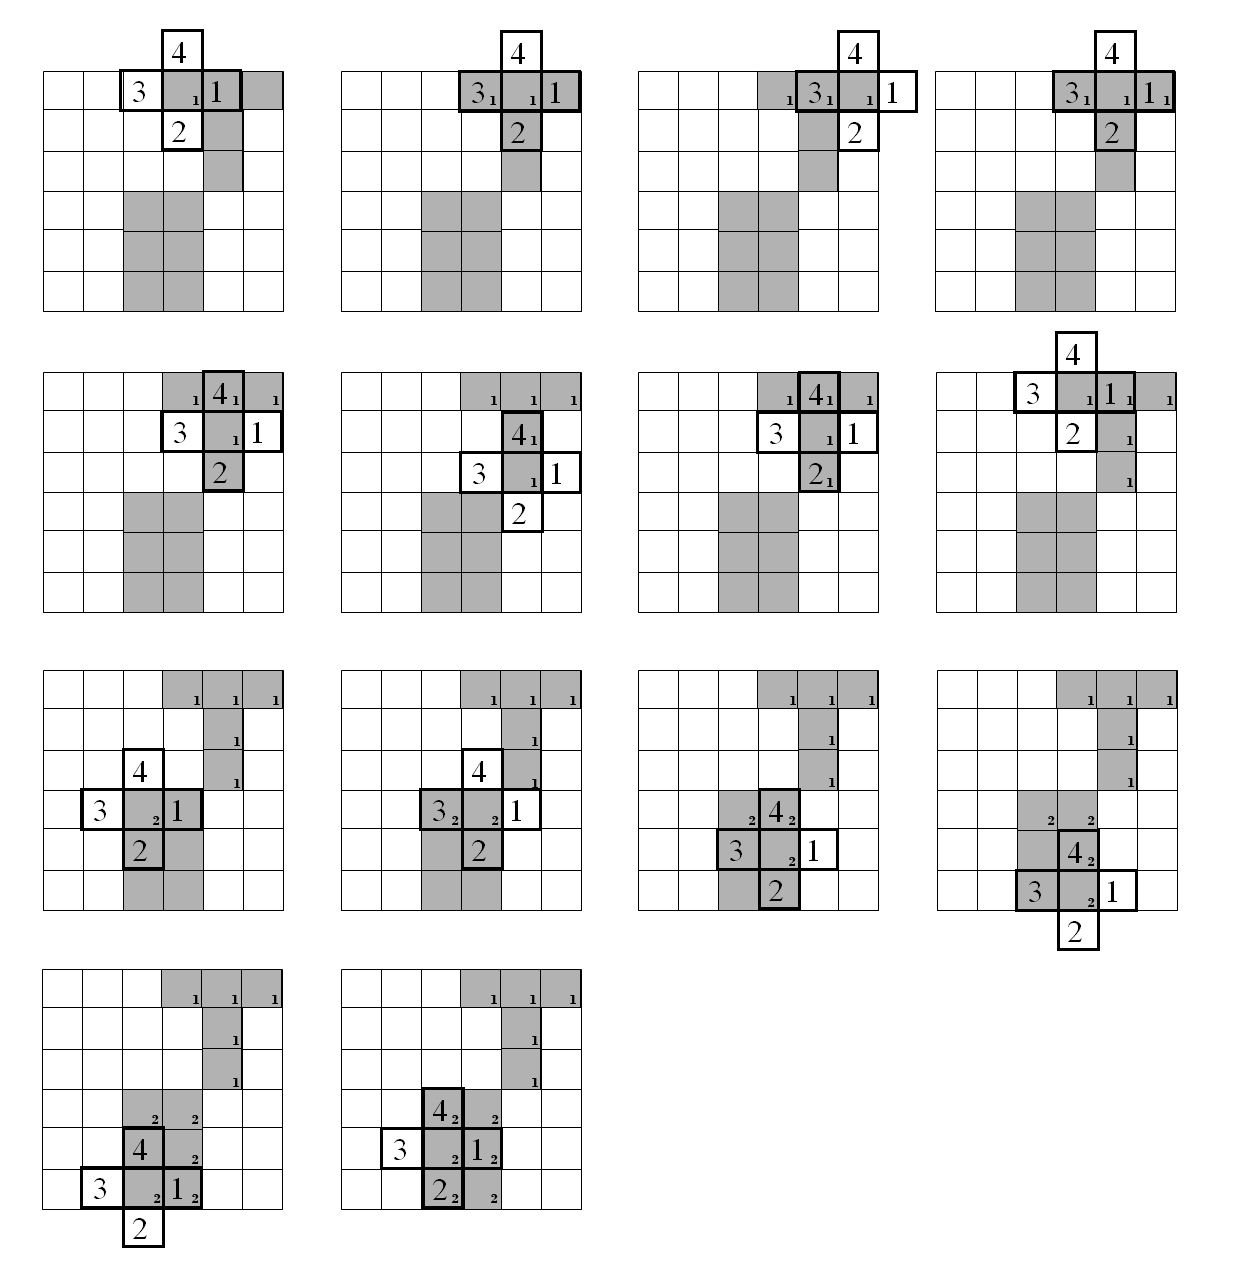
\includegraphics[width=0.75\textwidth]{Pictures/Theory/4connec_kernel.png}
\caption{4 connectivity labeling kernel detects 2 objects}
\label{fig:4connecK}
\end{figure}

\subsection{BLOB representation}
The classification of the BLOBs is made by creating a \textit{prototype model} of the object that we are looking for in order to state the features the BLOB should contain, and the deviations that would be acceptable. This process consists of two steps: Determining the features of the BLOB and matching the features with the prototype to determine if they are part of the type that we were looking for.

This means that a few features like the \textbf{area}, the \textbf{perimeter} and the \textbf{circularity} will be calculated.
\subsubsection{The features}

\begin{itemize}
\item Area
\\
\\
The importance of calculating features like the \textbf{area} of a BLOB is well understood if we keep in mind that one of the first steps while classifying the detected objects is to delete those that are bigger or smaller than the prototype. One way of doing this is by calculating the area of the BLOBs.

\item Bounding box and Bounding circle
\\
\\
Both \textbf{bounding box} and \textbf{bounding circle} are methods that operate in a similar way, as the particularity of these features is to find the minimum box or circle that can enclose the BLOB. The difference between these two besides the shape, is the way they operate. While the \textbf{bounding box} is the minimum rectangle and operates by finding four pixels; $x_max$, $x_min$, $y_max$ and $y_min$, which represent the minimum and maximum x and y values than can create a box that encompasses the BLOB. The \textbf{bounding circle} is the minimum circle and needs to find first the center of the BLOB.

\item Convex hull
\\
\\
The minimum convex polygon which contains the BLOB can be described as wrapping a piece of string tightly around the BLOB. Starting from the topmost pixel of the BLOB and searching to the right along a horizontal line and in a clockwise motion till it finds a BLOB pixel and creates the first side of the polygon.

\item Bounding box ratio
\\
\\
This is the height of the bounding box divided by the width, indicating the height-to-width ratio of the BLOB.

\item Compactness
\\
\\
The compactness of a BLOB is the ratio of the BLOBs area to the ratio of the bounding box.

\begin{equation}
	\begin{aligned}
	\text{Compactness}=\displaystyle\frac{BLOB's Area}{width\cdot{height}}
	\label{Compact}
	\end{aligned}
\end{equation}

\item Center of mass
\\
\\
In physics, the center of mass is the unique point where the mass of an object is equally distributed. The common example to explain this would be the place where you have to place your finger on an object in order to have it balanced.

The distribution of mass is balanced around the center of mass and the average of the weighted position coordinates of the distributed mass defines its coordinates. On a binary image, this center will be the average x and y positions of the object on the image.

Its coordinates can be found using the formula:

\begin{equation}
	\begin{aligned}
  		\ \text{Center of Mass} = \left\{ \begin{array}{ll}
         x_{c}=\displaystyle\frac{1}{N} \displaystyle\sum_{i=1}^N x_{i}\\
         y_{c}=\displaystyle\frac{1}{N} \displaystyle\sum_{i=1}^N y_{i}
        \end{array} \right . \ 
 	\end{aligned}
\end{equation} 


Where N is the number of pixels in the BLOB and $x_i$ and $y_i$ are the coordinates of each single pixel inside that BLOB. In some situation where we will need to calculate the center of mass of an object with annexed parts, a median filter or an erosion before using the previous formula would be appropriate.

\item Center of the bounding box
\\
\\
As the bounding box is a rectangle that surrounds the BLOB, the center of the bounding box is an approximation of the center of mass and can be found with the formula:

\begin{equation}
	\begin{aligned}	x_{bb}=x_{min}+\displaystyle\frac{x_{max}-x_{min}}{2}=x_{min}+\displaystyle\frac{x_{max}}{2}-\displaystyle\frac{x_{min}}{2}=\displaystyle\frac{x_{min}+x_{max}}{2}
	\label{BoundingBoxCenterX}
	\end{aligned}
\end{equation}

\begin{equation}	
	\begin{aligned}
	y_{bb}=y_{min}+\displaystyle\frac{y_{max}-y_{min}}{2}=y_{min}+\displaystyle\frac{y_{max}}{2}-\displaystyle\frac{y_{min}}{2}=\displaystyle\frac{y_{min}+y_{max}}{2}
	\label{BoundingBoxCenterY}
	\end{aligned}
\end{equation}


\item Perimeter
\\
\\
Scanning along the border of the BLOB and summing the pixels we obtain the length of the contour of the BLOB. In Image Processing, this could be done by using morphology techniques like erosion to get a smaller version of the object and then subtracting this to the input image in order to get the edges.

\item Circularity
\\
\\
Circularity is a very common shape factor that depends on the \textbf{Perimeter} and the \textbf{Area}. There are several ways to define how circular an object can be, but usually applying the ratio to get a value lower or equal to 1 will indicate how circular the BLOB is, where 1 is a complete circle.

\begin{equation}	
	\begin{aligned}
	{Circularity}=\displaystyle\frac{BLOB's \;\; Perimeter}{2 \; \sqrt{\mathstrut \: \pi \: \cdot \: {BLOB's \;\; Area}}}
	\label{Circularity}
	\end{aligned}
\end{equation}


After all the feature's extractions, a binary object can be defined by its features value that would be stored into a \textit{feature vector} in order to have a list where to start our BLOB's classification.

\end{itemize}


% IMAGE WITH OBJECTS AND TABLE WITH DATA

\begin{figure}[ht]
\begin{minipage}[b]{0.45\linewidth}
\centering
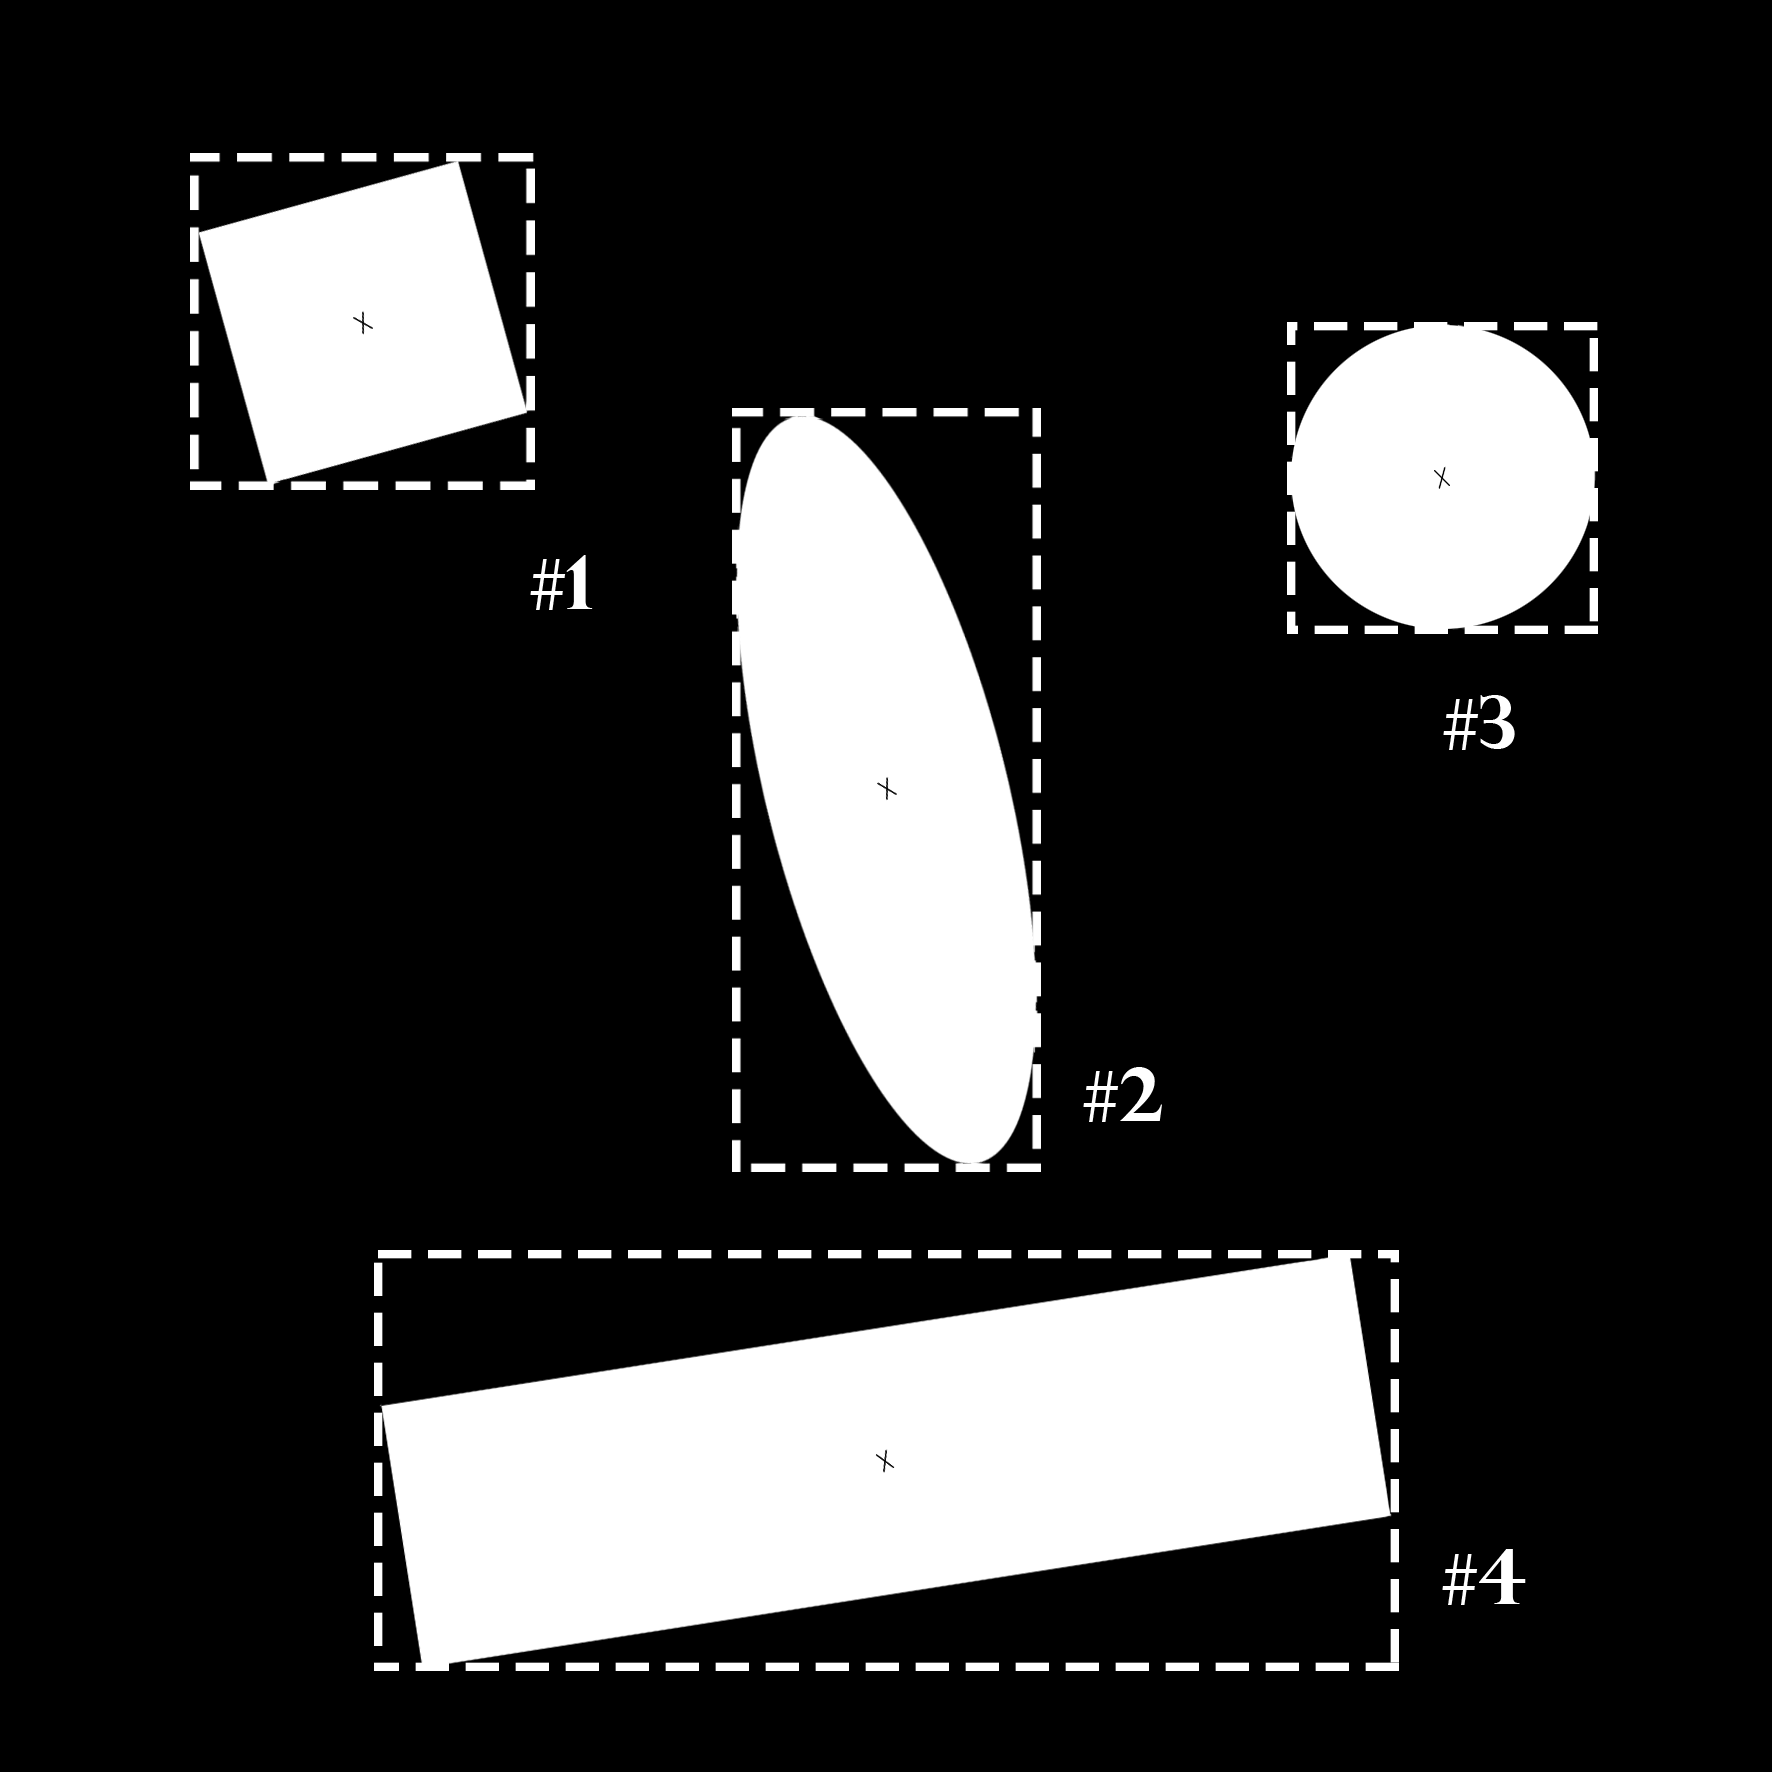
\includegraphics[width=1\textwidth]{Pictures/Theory/binary_image.png}
\end{minipage}
\hspace{0.5cm}	
\begin{minipage}[b]{0.45\linewidth}
\centering
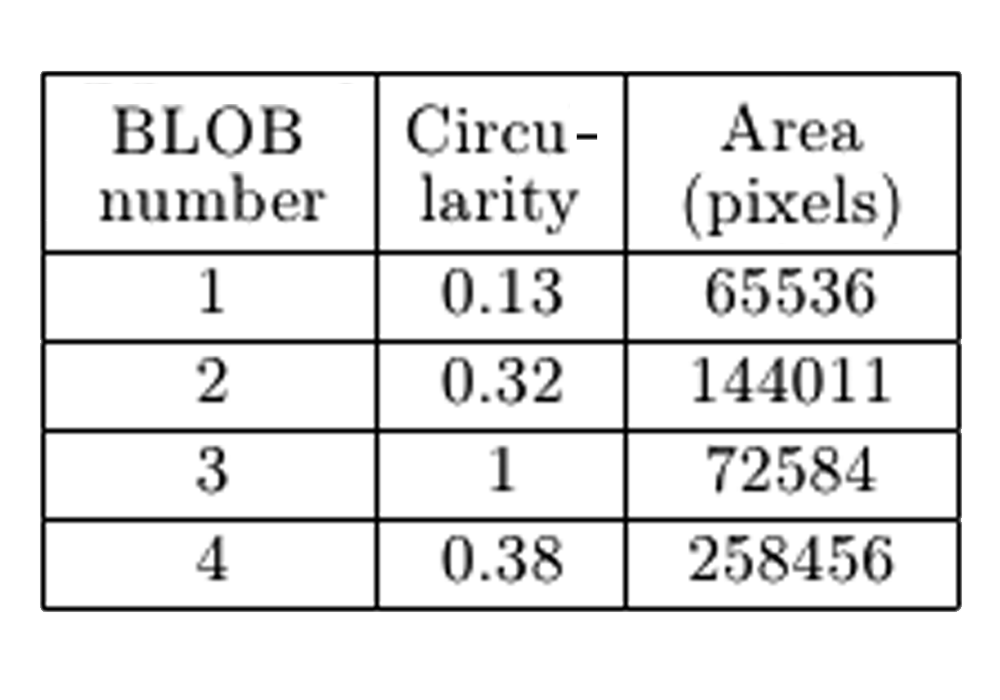
\includegraphics[width=1\textwidth]{Pictures/Theory/binary_image_table.png}
\end{minipage}
\label{fig:BinaryIm}
\caption{The figures above show a binary image with a Bounding Box and the Center-of-Mass. The table shows two other features that can be calculated (the \textbf{\textit{perimeter}} and the \textbf{\textit{area}})}
\end{figure}

%%%%%%%%%%%%%%%%%%%%%%%%%%%%%%%%%%%%%%%%%%%%%%%%%%%%%%%%%%%%%%%%%%%%%%%%%%%%%%%%

\subsection{BLOB classification}
Once we have extracted and represented each object on the binary image by its features, we need to determine the minimum characteristics that the object has to comply to in order for it to be selected.
For this reason, we will define a \textit{prototype model} based on ideal measurements that is used as a reference to which the extracted values are compared. As the real object will not be perfect, a deviation is needed to create a tolerance range.
Using two features like the circularity and the area we will create a frame, also known as a \textit{box classifier}, and every object belonging to that \textit{feature space}, also know as \textit{decision region}, will then be understood as a desired object.

Another way to achieve this would be to create a \textit{statistical classifier} using means and variances of the features, where the task would be to measure the distance between a new feature vector and the prototype. The smaller the distance between those two, the more likely the object will be part of the same type. But before getting to this point, we need to threshold the distance and consequently have a binary decision region like the \textit{box classifier}.
This time, the region will not be a rectangle but an ellipse, and is commonly known as the \textit{weighted Euclidean distance}.

\begin{equation}	
	\begin{aligned}
{WED(\vec{f}_{i} \; , \: prototype)} \: = \: \sqrt{\mathstrut \:  \displaystyle\frac{(f_{i}(cir) \: - \: mean(cir))^2}{variance(cir)} \: + \: \displaystyle\frac{(f_{i}(area) \: - \: mean(area))^2}{variance(area)}}
\label{Euclidean}
	\end{aligned}
\end{equation}

The final result is the distance between the vector {$\vec{f}_{i}$} and the prototype. The values of {$f_{i}(cir)$} and {$f_{i}(area)$} correspond to the circularity and the area of every object found on the binary image. For an image with a number of N different features, the result would be obtained by summing:


\begin{equation}	
	\begin{aligned}
{WED(\vec{f}_{i} \; , \: prototype)} \: = \: \displaystyle\sum_{i=1}^N \: \: \sqrt{\mathstrut \:  \displaystyle\frac{(f_{i}(m_{j}) \: - \: mean(m_{j}))^2}{variance(m_{j})}}
\label{Euclidean1}
	\end{aligned}
\end{equation}

Where {$m_{j}$} is the {$jth$} feature. When the variances of the features are the same all along the list of values, we can ignore it and calculate the Euclidean distance (ED), where the region is a circle in 2D.

\begin{equation}	
	\begin{aligned}
{ED(\vec{f}_{i} \; , \: prototype)} \: = \: \displaystyle\sum_{i=1}^N \: \sqrt{\mathstrut (f_{i}(m{j}) - mean(m_{j}))^2}
\label{Euclidean2}
	\end{aligned}
\end{equation}

But before we can calculate the distances, we need to normalize the values to the same scale and interval.

Therefore, the Area would be done by:

\begin{equation}	
	\begin{aligned}
{Area \: feature} \: = \: min \begin{Bmatrix} \displaystyle\frac{Area\:of\:BLOB}{Area\:of\:Model}, & \displaystyle\frac{Area\:of\:Model}{Area\:of\:BLOB}\end{Bmatrix}
\label{NormArea}
	\end{aligned}
\end{equation}

The Circularity can also be normalized in the same:

\begin{equation}	
	\begin{aligned}
{Circularity \: feature} \: = \: min \begin{Bmatrix} {Circularity}, & \displaystyle\frac{1}{Circularity}\end{Bmatrix}
\label{NormCirc}
	\end{aligned}
\end{equation}